% Dokumenteinstellungen
% ======================================================================

% Die Dokumentklasse definiert die Art des Dokuments
% und seine Grundeigenschaften
\documentclass[11pt,a4paper]{scrartcl}		% [Schriftgröße 10, Textbereich Din A4] {Dokumentart Artikel}


% Zusätzliche (aber sinnvolle) Pakete laden
% ======================================================================
% Pekete fügen verschiedene Funktionen zu LaTeX hinzu.
% ganz ohne Pakete wäre Latex gerade mal etwas besser als notepad...
\usepackage[a4paper]{geometry}				% DIN-A4 Größe des Papiers; sollte mit der Ausdehnung des Textes in documetnclass übereinstimmen.
\usepackage[utf8]{inputenc}					% Zeichenkodierung UTF-8 falls Probleme wegen utf8 auftreten, utf8 durch utf8x ersetzen
\usepackage[T1]{fontenc}
\usepackage{lmodern}
\usepackage{amsmath}						% erlaubt mathematische Formeln
\usepackage[english]{babel}					% Deutsche Sprache und Silbentrennung
\usepackage{amssymb}						% Verschiedene Symbole
\usepackage{graphicx}						% Zum Bilder einfügen benötigt
\usepackage{hyperref}						% Sprunglinks für Überschriften, Fußnoten und Weblinks

%Eigenes

\usepackage{subfig}							% Subfloat Benutzung, Unterteilung für Bilder

\usepackage[numbers,square]{natbib}
\bibliographystyle{alphadin}%plaindin}%unsrt}%alphadin}
\usepackage{gensymb}
\usepackage{setspace}
\usepackage{geometry}
\geometry{a4paper,left=2.5cm,right=2.5cm}

\usepackage{siunitx}
\usepackage{booktabs}
\usepackage{eurosym}

\usepackage[shortlabels]{enumitem}

\usepackage{fixltx2e}  % Für \textsubscript{}

\usepackage{tabularx}
\newcolumntype{L}[1]{>{\raggedright\arraybackslash}p{#1}}
\newcolumntype{R}[1]{>{\raggedleft\arraybackslash}p{#1}}
\newcolumntype{C}[1]{>{\centering\arraybackslash}p{#1}}

\usepackage{longtable}

\usepackage{pdfpages}

\usepackage{pstricks}	% Erstellung von Plots
\usepackage{pst-plot}

\usepackage{placeins}

% Dokumentbeginn
% ======================================================================
% Ab hier beginnt das eigentliche Dokument.
% Alles was danach folgt wird im fertigen PDF angezeigt.

\begin{document}


% Titelblatt
% ===========================================

\begin{titlepage}
	
	\singlespacing
	\begin{center}
	
		\quad
		\vspace{1cm}
	
		\Large{\textbf{Project Work\\Cyber-Physical Systems}}
	
		\vspace{1.5cm}
	
		\huge{\textbf{Autonomous Aerobatics on\\Commanded Paths}}
	
		\vspace{1.5cm}
	
		written by
		
		\vspace{1.5cm}
	
		\Large{\textbf{Youlin Gao\\Anthony Blanc\\Andreas Bruckmeier}}
	
		\vfill
		
		submitted at the\\
		Institute for Real-Time Computer Systems\\
		Technische Universität München,\\
		to\\
		Prof. Marco Caccamo

		\vspace{1cm}		
		
		Date: 6\textsuperscript{th} March 2016
	
	\end{center}
	
\end{titlepage}

\setstretch{1.2}


% Inhaltsverzeichnis   (Überschriften werden automatisch in das Inhaltsverzeichnis aufgenommen.)
% ===========================================
\newpage
\tableofcontents	

\vspace{2.0cm}

% Abbildungsverzeichnis
% ===========================================

%\renewcommand{\listfigurename}{}
\listoffigures
%{\def\section*#1{}\listoffigures}


% Textbeginn
% ================================================================================
% ================================================================================


% Neue Seite
% ===========================================
\newpage
	

\section{Overview}

As a part of the Cyber-Physical Systems course in WS15/16, a controller structure for an aircraft in a simulation environment was realised, performing autonomous aerobatics on commanded paths.
In this report, the controller structure is presented in Chapter~\ref{ch_Details}, and performance results are shown in Chapter~\ref{ch-Results}.
Before this, an overview of the working principle and the features of the controller are given, and the underlying work is clarified.

\medskip






\subsection{Working Principle and Features}

Control target of the presented system is to follow a path as a function of time in 3-dimensional space.
The aircraft's aim is to fly along this commanded path by determining the deviation from the given trajectory and thereout calculating acceleration commands which are the inputs of the aircraft's actuator controllers.

\textbf{Figure~\ref{fig_complete_structure}} depicts the complete control structure of the aerobatic controller. 
With the position data from the desired trajectory and with actual position signals of the aircraft, the desired acceleration to follow the path is computed.
After considering the gravity, the desired acceleration is handed to the control structure where the acceleration in body frame is used as the control variable for the aileron-, elevator-, and rudder-controllers.
Also, with the position data, the delay of the aircraft from the desired position is determined, and by considering a \textsl{look-ahead distance} which forces the aircraft to lag behind the path by a specific distance, the throttle is controlled with this information.

The resulting steering signals, computed by the control structure, are handed to the simulation environment which simulates the physical reaction of the aircraft and then hands back measurement results of its virtual sensors.
These signals are processed and provided to the control structure. 
A feature of the \texttt{Signal Processing} is the estimation of the aircraft's position with only accelerometers and gyrometers when there is no available GPS-signal as it is in inverted flight attitude.

\begin{figure}[!h]
  \begin{center}
  	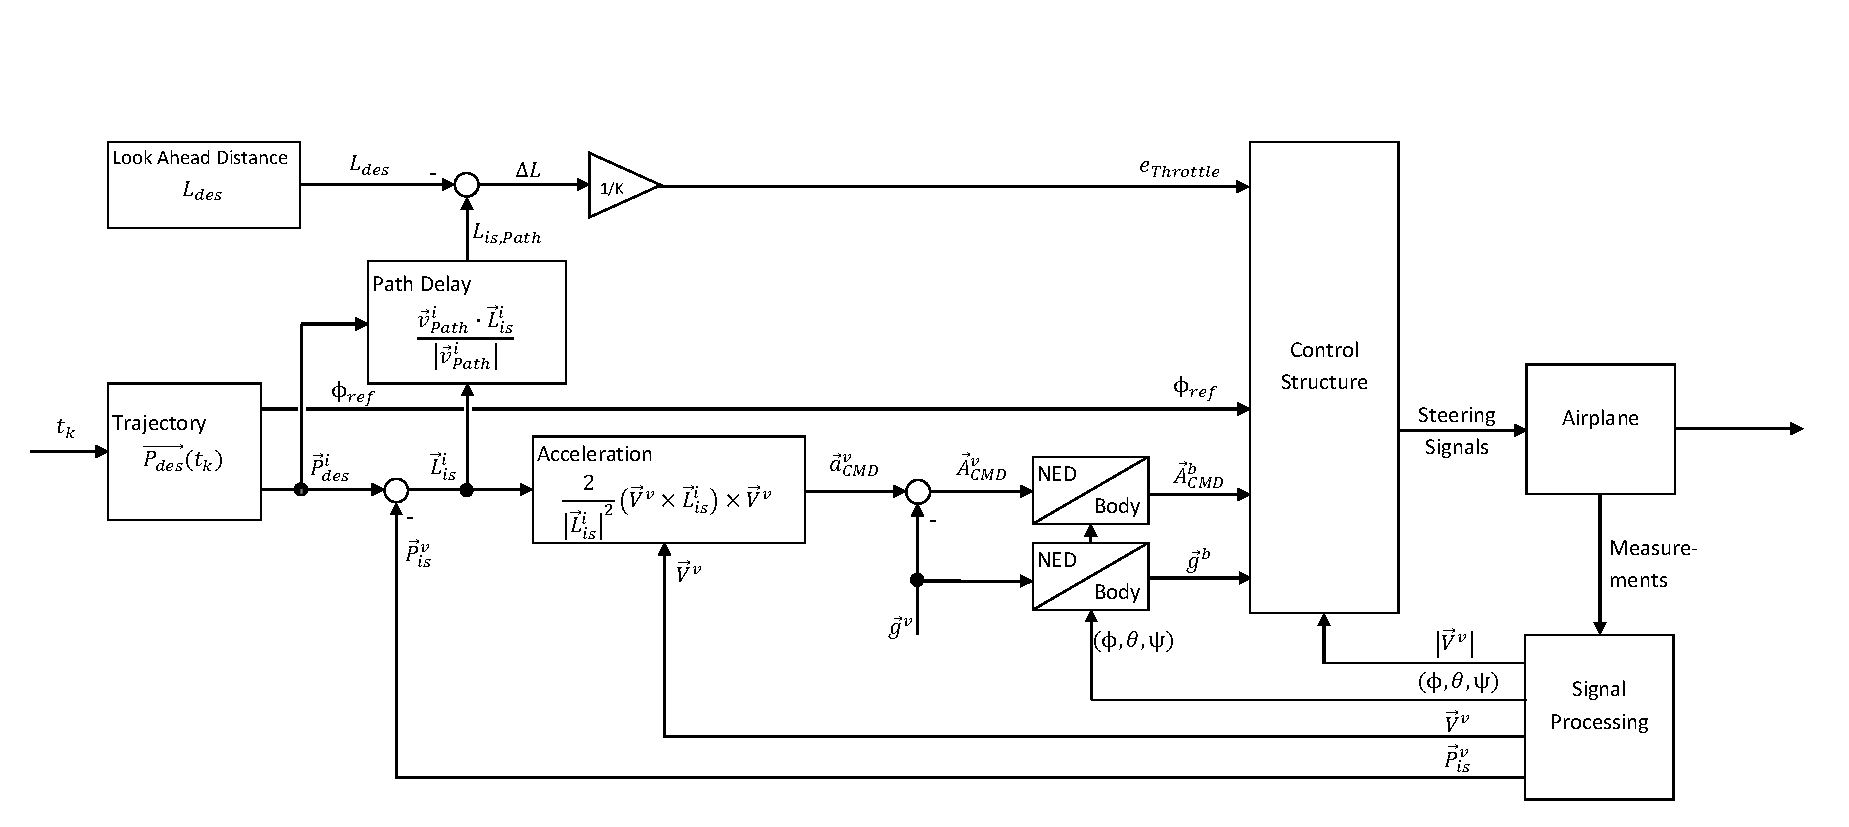
\includegraphics[width=18.8cm, angle=90]{pictures/complete_structure.pdf}
  \end{center}
  \caption{Overview of the control structure of the aerobatic controller.}
  \label{fig_complete_structure}
\end{figure}


\subsection{Underlying Work}

The control structure, implemented and presented in this project work, is based on the work of Sanghyuk Park\cite{Park.2012} and modified by establishing the desired path depending on time plus determining the path delay in order to control the throttle.

The estimation of the aircraft's position signal is implemented after a method which is, at the time of handing in this report, not yet published. We got the access ahead of the release by our tutor \cite{Dantsker.2016}.

\medskip





\section{Details}\label{ch_Details}

In the following, each part of the control structure (compare Figure~\ref{fig_complete_structure}) is presented in detail.

\medskip





\subsection{Interface with the Simulation Environment}

The connection of our program with the simulation environment takes place at the beginning of each program run, when sensor data is handed over and at the end of each run, when commands for the actuators are given to the aircraft.

In the code, the function~\textsf{calculateStateVariables} reads the sensor data of the aircraft to our part of the software.
At the end of each program run, the four steering signals for the actuators throttle, aileron, rudder, and elevator are given to the simulation environment in the function~\textsf{generateOutSignals}.

\medskip




\subsection{User Interface}

We have implemented an user interface which enables a communication with the aircraft controller via an USB connection with the controller board. 
We used the program \texttt{hterm} for communicating with the controller over a COM-Port.
In the code, the function \textsf{API\_interpretate\_chain} cares for the interpretation of the user commands and the instruction transfer.
The interface enables the user to modify controller parameters and flight special pre-established paths at run time:

\medskip

Sending the letter \texttt{'h'} prints help instructions and explanations how to use the interface.

\medskip

We have implemented a few (aerobatic) paths that can be commanded to the aircraft. 
These trajectories are managed as a state machine in function~\textsf{Trajectory.cpp} and are depicted graphically in \textbf{Figure~\ref{fig_state-machine}}. 
Every state corresponds to a different path. Some of the states are \textsl{'unstable'} due to a finite duration of the path. The arrows in the figure indicate the subsequent state. 
Paths, represented as \textsl{'stable'} states, have an unlimited duration and are active as long as no other command occurs.
With following commands, starting with \texttt{'f'}, the commanded path can be changed (Details on each path are given in the following section):

\begin{tabbing}
	\hspace{2cm} \= \hspace{4cm} \= \hspace{3cm} \kill
	\> 0. Take Off \> \texttt{ft} \\	
	\> 1. Circle \> \texttt{fc} \\	
	\> 2. Looping\> \texttt{fl} \\	
	\> 3. Glide Eastwards \> \texttt{fg} \\
	\> 4. Roll Manoeuvre \> \texttt{fr} \\		
	\> 5. Glide Westwards \> \texttt{fb} \\	
	\> 6. Half Circle \> \texttt{fh} \\	
	\> 7. Climb Up \> \texttt{fc} \\	
	\> 8. Snake Flight \> \texttt{fs} \\		
\end{tabbing}



\medskip

Furthermore, with the user interface variables, changing the behaviour of the control structure, can be adjusted during flight, namely the gains~$K$ of the PID-controllers and the \textsl{look-ahead distance}~$L_{des}$:

\begin{tabbing}
	\hspace{2cm} \= \hspace{6cm} \= \hspace{7cm} \kill
	\> Edit Throttle-PID gains \> \texttt{et-\#$K_P$\#-\#$K_I$\#-\#$K_D$\#} \\
	\> Edit Aileron-PID gains \> \texttt{ea-\#$K_P$\#-\#$K_I$\#-\#$K_D$\#} \\
	\> Edit Rudder-PID gains \> \texttt{er-\#$K_P$\#-\#$K_I$\#-\#$K_D$\#} \\
	\> Edit Elevator-PID gains \> \texttt{ee-\#$K_P$\#-\#$K_I$\#-\#$K_D$\#} \\
	\> Edit \textsl{look-ahead distance} \> \texttt{l-\#$L_{des}$\#} 
\end{tabbing} 
with 
\begin{tabbing}
	\hspace{2cm} \= \hspace{3cm} \= \hspace{7cm} \kill
	\> \#$K_P$\# \> Value of the \textsc{Proportional}-gain \\
	\> \#$K_I$\# \> Value of the \textsc{Integral}-gain \\
	\> \#$K_D$\# \> Value of the \textsc{Derivative}-gain \\
	\> \#$L_{des}$\# \> Value of the \textsl{look-ahead distance} \\
\end{tabbing}
\noindent
Note: In the code, it is possible to change the \textsl{separation character}. We have chosen \texttt{\'-\'} but it might be modify by changing the defined value \textsf{separation\_char}.

\medskip
\noindent
As demonstration, two commands are given how to change controller gains:
\begin{itemize}
\item 
\texttt{et-1.56-2.55-0} : Edit the Throttle-PID with the Proportional-gain equal to 1.56, the Integral-gain equal to 2.55 and the Derivative-gain equal to 0.0.
\item
\texttt{ea-7.01-0.55-0.22} : Edit the Aileron-PID with the proportional-gain equal to 7.01, the Integral-gain equal to 0.55 and the Derivative-gain equal to 0.22.
\end{itemize}

\begin{figure}[bt]
  \begin{center}
  	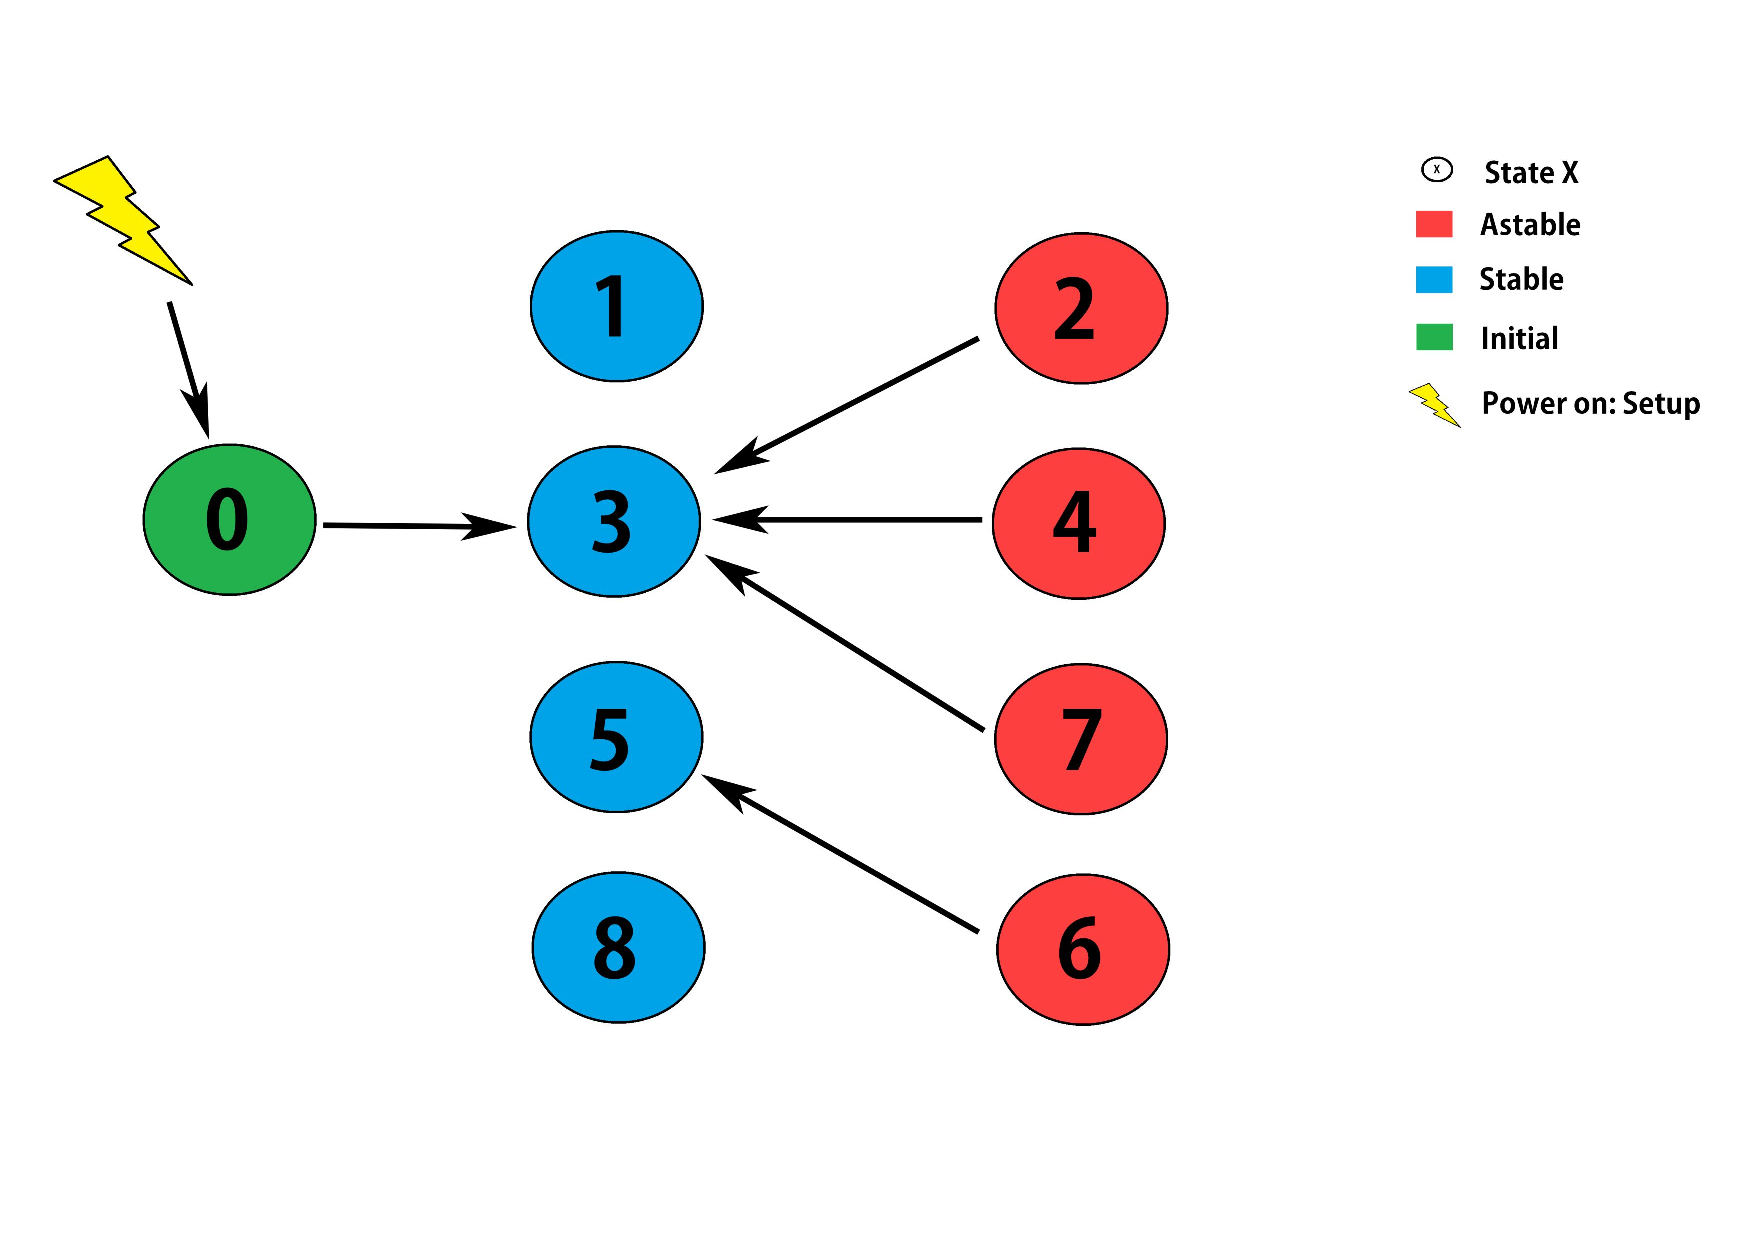
\includegraphics[width=11cm]{pictures/StateDiagramme_liason.pdf}
  \end{center}
  \caption{Overview of implemented paths depicted as a State Machine.}
  \label{fig_state-machine}
\end{figure}

\bigskip

It is also to mention, that we introduced two time signals, the \textsl{hardware time} and the \textsl{relative time}.
The hardware time is the time since the start-up of the aircraft controller whilst relative time measures the time passed since the last restart of the aircraft in the simulation environment.
A restart brings back the aircraft to the initial position position on the start field, and thus we make sure to reset the desired path plus the relative time, too, in order to bring back the system to a initial state without the need to reset the controller.
In the code, this functionality is implemented in lines 164--178 in \textsf{Autopilot.pde}.

\medskip




\subsection{Path Generation} \label{ch-Path-Generation}

Our commanded paths are designed in function~\textsf{Trajectory.cpp}. 
The idea of designing a trajectory, the aircraft should follow, is a stepwise addition of a position vector at every time step
\begin{equation}
\vec{P}^i_{des}(t_k)=\vec{P}^i_{des}(t_{k-1}) + \Delta\vec{P}^i(t_k) \cdot \Delta T
\end{equation}
which can be considered as a integration process of the position with the \textsl{velocity vector}~$\Delta\vec{P}^i(t_k)$.
As described later in Chapter~\ref{ch-control-variables}, the aircraft is controlled that it will stay behind the commanded path in a distance equal of about one second leading to a vector $\vec{L}_{is}^i = \vec{P}_{des}^i - \vec{P}_{is}^i$ which controls the aircraft like dragging the string of a kite.

\medskip

Currently we have nine different acrobatic paths implemented. They can be divided into two categories, into stable flight paths and temporary flight paths (compare Figure~\ref{fig_state-machine}).

\subsubsection*{Stable Paths}
Stable flight paths serve as a kind of default flying states.
They are maintained when undisturbed, and can be interrupted at any time by other flying modes. To change the commanded path, one enters a new path command, given in previous section, in the console.
Details of our implemented paths are listed here:

\begin{itemize}

\item
\texttt{fg}: Glide Eastwards or Go-Straight mode. The airspeed is set to $\SI{50}{ft\per\second}$ in direction east.

\item
\texttt{fb}: Glide Westwards mode. The airspeed is set to $\SI{50}{ft\per\second}$ in direction west.

\item
\texttt{fc}: Circle mode. With a radius of $\SI{70}{ft}$, a circle is flown. 
The radius and speed of the aircraft can be modified in function~\textsf{Trajectory.cpp}. Additionally, the path commands a slight inclination speed of $\SI{1}{ft\per\second}$ to avoid a crash when manoeuvring at a low altitudes.

\item
\texttt{fs}: Snake mode. This path goes into east-direction, with a left/right snake sinusoidal turn in north/south direction. The radius is set to $\SI{50}{ft}$.

\end{itemize}

\subsubsection*{Temporal Aerobatic Paths}

Paths, which have certain durations and are executed from beginning until its end, are  temporal ones. After performing a temporal aerobatic path, the aircraft changes back into a default flying state, such as flying forward or backward. 
Details of temporal aerobatic paths are:

\begin{itemize}

\item
\texttt{ft}: Take Off mode. In this mode the aircraft has a relatively low climb rate for a safe take Off.

\item
\texttt{fl}: Looping mode. The aircraft performs a backward-direction loop by first climbing up and flipping over. A whole barrel loop can be achieved by two backward-direction loopings. 

\item
\texttt{fr}: Roll mode. The aircraft rolls over 360 degrees for one time in this mode. The aircraft finishes rolling in two steps, each turn is 180 degrees.

\item
\texttt{fh}: Half Circle mode. The aircraft, going westwards, flies a half-circle in a downward looping manner and then flies straight eastwards.

\item
\texttt{fc}: Climb Up mode. The Take Off mode has a low climb rate, in this mode, the climb rate is larger in order to have a quicker climb up.

\end{itemize}

The aerobatic flight durations are defined and can be changed in function~\textsf{Trajectory.cpp}. In each gesture's sub-function, parameters, such as speed, climb rate, or roll rate, can also be changed.

\medskip





\subsection{Processing of Control Variables} \label{ch-control-variables}

Now, we describe the computation of the variables, handed to the \texttt{Control Structure}, given the state variables, provided in function~\textsf{calculateStateVariables}, and the desired path, as described in Chapter~\ref{ch-Path-Generation}.

\subsubsection*{Computing the Desired Acceleration}

As an essential part of the aerobatic controller, a \textsl{look-ahead distance}~$\L_{des}$ is introduced which effects the system to control the aircraft to lag behind the desired path by an adjustable distance.
This guarantees the difference between desired and actual position of the aircraft 
\begin{equation}
\vec{L}_{is}^i = \vec{P}_{des}^i - \vec{P}_{is}^i
\end{equation}
to be greater than zero and leading to acceleration commands 
\begin{equation}
\vec{a}_{CMD}^v = \frac{2}{|\vec{L}_{des}^i|^2}\left(\vec{V}^v \times \vec{L}_{is}^i \right) \times \vec{V}^v
\end{equation}
being moderate and viable by the aircraft.
This acceleration command is then subtracted by the gravity constant
\begin{equation}
\vec{A}_{CMD}^v = \vec{a}_{CMD}^v - \vec{g}^v
\end{equation}
and handed to the Control Structure in body frame:
\begin{equation}
\vec{A}_{CMD}^b = \mathcal{R}_i^b(\phi,\theta,\psi) \cdot \vec{A}_{CMD}^v \quad .
\end{equation}

\medskip




\subsubsection*{Determining the Desired Speed}\label{ch-Determ-Desired-Speed}

The desired speed of the aircraft is given implicitly with the desired path and can be gathered by calculating the derivative of $\vec{P}_{des}^i$:
\begin{equation}
\vec{v}_{Path}^i(t_k) = \frac{\vec{P}_{des}^i(t_k)-\vec{P}_{des}^i(t_{k-1})}{\Delta T}\quad .
\end{equation}

But the desired speed is not the control variable of the throttle controller. As shown in Figure~\ref{fig_complete_structure}, the input for the throttle controller is $\Delta L$ which is the distance of the aircraft from the desired position with respect to the \textsl{look-ahead distance}~$L_{des}$ and is computed by
\begin{equation}
\Delta L = \frac{\vec{v}_{Path}^i \cdot \vec{L}_{is}^i}{|\vec{v}_{Path}^i|}-L_{des} = L_{is,Path}-L_{des} \quad .
\end{equation}
Here, $L_{is,Path}$ is the distance of the aircraft concerning/on the desired flight direction expressed in $\vec{v}_{Path}^i$.
This relation is shown graphically in \textbf{Figure~\ref{fig_explanation-diagram-throttle}}. The inner structure of the component \texttt{Path Delay} is depicted in \textbf{Figure~\ref{fig_Path_Delay}}.
Finally, $\Delta L$ is divided by a constant value~$K$ and handed to the throttle controller as input $e_{Throttle}$ (see Figure~\ref{fig_Control-Structure}).

\begin{figure}[bth]
  \begin{center}
  	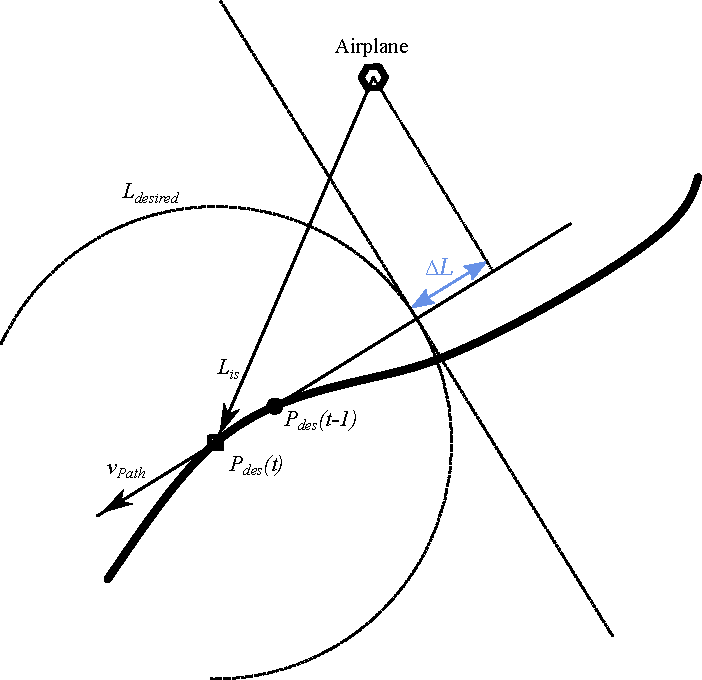
\includegraphics[width=9cm]{pictures/explanation-diagram-throttle.pdf}
  \end{center}
  \caption{Determination of the input for the throttle-controller $\Delta L$.}
  \label{fig_explanation-diagram-throttle}
\end{figure}

\begin{figure}[tbh]
  \begin{center}
  	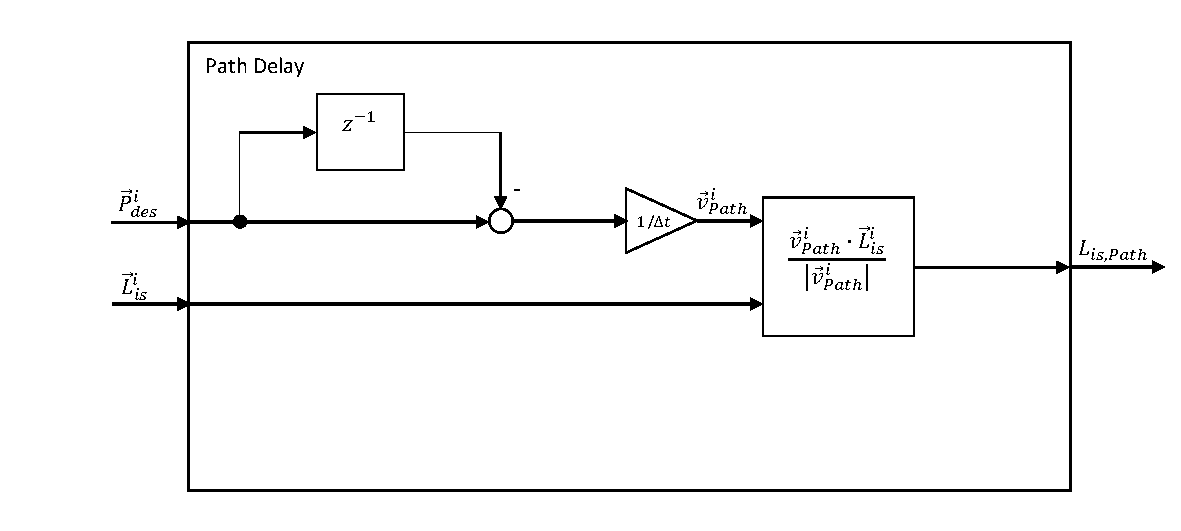
\includegraphics[width=14cm]{pictures/Path_Delay.pdf}
  \end{center}
  \caption{Inner structure of the component \texttt{Path Delay}.}
  \label{fig_Path_Delay}
\end{figure} 

With this control mechanism, the aircraft will adjust the throttle in order to always stay behind the desired position by the length of the \textsl{look ahead distance}~$L_{des}$ which is the intersection of the desired flight direction~$\vec{v}_{Path}^i$ and the circle of $L_{des}$ as shown in Figure~\ref{fig_explanation-diagram-throttle}. In this point, $\Delta L$ will become zero, which is the control target of the control structure (of course, the whole tangent of the intersection point will meet the control target of $\Delta L = 0$ but the rest of the control structure will force the aircraft onto the desired path and thus to this one intersection point).  

\medskip





\subsection{Control Structure}

In the \texttt{Control Structure}, the four actuators of the aircraft, namely throttle, aileron, rudder, and elevator, are regulated by PID-controllers with an error~$E$ as input value:
\begin{equation}
output(t) = K_p \cdot E(t) + K_i \cdot \int_{t_0}^t E(\tau)\, \mathrm{d}\tau + K_d \cdot \frac{\mathrm{d}}{\mathrm{d}t}E(t)\quad .
\end{equation}

\subsubsection*{Throttle}
The input error of the throttle is the sum of current aircraft velocity~$|\vec{V}^v|$ and the distance of the aircraft~$e_{Throttle}$, lagging behind its desired position, as described in Section~\ref{ch-Determ-Desired-Speed}:
\begin{equation}
E_{throttle} = |\vec{V}^v| + e_{Throttle} \quad .
\end{equation} 
The aircraft velocity term is for keeping the engine speed at the desired level, only the error term can increase or decrease the engine speed.

\subsubsection*{Aileron}
The aileron controller is implemented as described in the work of S.~Park\cite[p.~71]{Park.2012}.
A reference vector~$\hat{e}_{roll}$, always pointing out of the roof of the aircraft, is compared with the acceleration command~$\vec{A}_{CMD}^b$. 
The control target is to let both vectors point into the same direction (this is shown graphically in the paper of S.~Park on page~70~\cite{Park.2012}.
Mathematically, this is achieved with following equation:
\begin{equation}
E_{aileron}=\arcsin\left(\hat{e}_{roll} \times \frac{\vec{A}_{CMD}^b}{|\vec{A}_{CMD}^b|}\right)_x
\end{equation}
The reference vector~$\hat{e}_{roll}$ can be modified by the angle~$\phi_{ref}$. At the value of $\phi_{ref}=90\degree$, $\hat{e}_{roll}$ is pointing out of the right wing of the aircraft; at $\phi_{ref}=180\degree$, the reference vector is pointing out of the fuselage.
Altering the angle of the reference vector can be used for performing a roll manoeuvre.

\subsubsection*{Rudder and Elevator}
Rudder and elevator are controlled with the acceleration command~$\vec{a}_{CMD}^b$, which does not contain the gravity term~$\vec{g}^b$.
The rudder control takes the y-component as input, and the elevator control uses the z-component:
\begin{equation}
E_{rudder}=(\vec{a}_{CMD}^b)_y\quad , \quad E_{elevator} = (\vec{a}_{CMD}^b)_z
\end{equation}

The \texttt{Control Structure} is depicted in symbolic form in \textbf{Figure~\ref{fig_Control-Structure}}.

\begin{figure}[tbh]
  \begin{center}
  	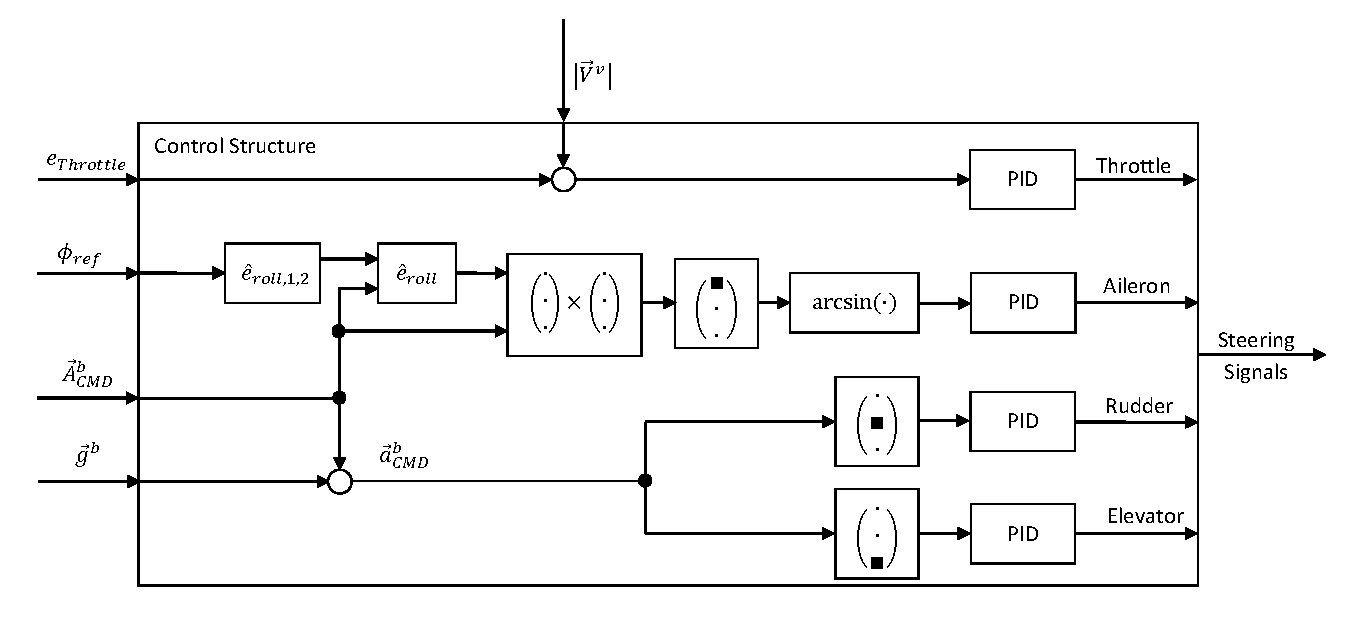
\includegraphics[width=15cm]{pictures/PID.pdf}
  \end{center}
  \caption{Inner structure of the component \texttt{Control Structure}.}
  \label{fig_Control-Structure}
\end{figure}


\medskip






\subsection{GPS Signal Estimation}

In the case of an inverted flight attitude, a GPS-signal cannot be received due to GPS receivers not pointing to the sky.
Therefore, the position of the aircraft has to be estimated with signals from measuring instruments, still available, which is the data from accelerometers and gyroscopes.
However, in the simulation, position data is always provided perfectly, so an inverted flight attitude has first to be detected and position signals have then to be ignored in order to realise a \textsl{real} GPS-signal.

\smallskip

So, the function~\textsf{NoSignalAvailableGPS} is implemented, observing the euler angles of the aircraft, wherewith the flight attitude of the aircraft is depicted.
As soon as the roll angle~$phi$ or pitch angle~$\theta$ is according to amount greater than $60\degree$, this function activates the \textsl{position estimation} which overwrites the ideal position signals.

\smallskip

The \textsl{position estimation}-principle, implemented in the function \textsf{estimateStateVars}, is a method of integration \cite{Dantsker.2016}.
First, the derivatives of the Euler angles are computed with the available rotation rates by changing the coordinate frame. 
Then, the Euler-derivatives are time-step integrated with the previous values to obtain the new Euler angles, e.g.:
\begin{equation}\label{eq-integration}
 \phi_{t_k} = \frac{1}{2}(\dot{\phi}_{t_k}+\dot{\phi}_{t_{k-1}})\cdot \Delta T + \phi_{t_k} \quad .
\end{equation}

In the next step, the acceleration of the aircraft is depicted with the data of the accelerometer~$A$ plus data of the rotation rates~$pqr$, where $\mathbf{C_r}$ offsets the location of the IMU and $\mathcal{R}_b^i$ is the transformation from body frame to inertial frame:
\begin{equation}
\ddot{P^i}(t_k)= \mathcal{R}_b^i(\phi,\theta,\psi)(t_k)\cdot A(t_k) + \mathbf{C_r} \cdot \left[ pqr(t_k) \times uvw(t_{k-1})\right] \quad .
\end{equation}
Here, $uvw$ is the velocity of the aircraft in body frame:
\begin{equation}
uvw(t_k) = \mathcal{R}_i^b(\phi,\theta,\psi)(t_k) \cdot \dot{P^i}(t_k) \quad .
\end{equation}

With the same time-step integration method as shown in Equation~\ref{eq-integration}, the aircraft-velocity, and with a further integration step, the position of the aircraft can be obtained:
\begin{equation}
\ddot{P^i} \rightarrow \dot{P^i} \rightarrow P^i \quad .
\end{equation}

\smallskip

As soon as the aircraft is able to receive a GPS-signal again, the estimation is switched off and the ideal position data is used.


\medskip





\section{Results}\label{ch-Results}


In summary, the presented and implemented control structure showed very good results for various aerobatic manoeuvres which are shown in the following.

\subsubsection*{Restraints}

But beforehand, it is to mention that the rudder was not activated as the results were recorded.
The reason was a faulty adapter software which caused a disconnection with the controller after a few seconds of flight. Instead, we used a stable working adapter software which did not support the control of the rudder.

Also, the GPS signal estimation could not be activated due to imprecise estimation results.
The reasons were the lack of information about the used units of the measurement data and the position of the accelerometers in the aircraft which has to be considered in a compensation term.

\subsubsection*{Analysis of flown Trajectories}

In this project, we adopted \textsc{Matlab} to help us analysing our flown trajectories. 
We were able to compile 3-dimensional recordings of the flown path enabling us to find possible errors in control or path parameter designs.

The \textsc{Matlab} code and our recorded results were released together with the code of the aerobatic controller in the \textsl{Analysis}-folder . 
Basically we compare 3 sets of data recorded with the program \texttt{hterm}: The desired path, the real flown trajectory, and the $\vec{L}_{is}^i$ vector. 

\medskip

In \textbf{Figure~\ref{fig_circle}}, the plots of the desired and the real trajectory of the Circle Path are shown. 
The desired path is shown above and the real trajectory is underneath. 
We can see that the aircraft adjusted itself to the sharp turn quickly and followed the desired path quite accurate. The take off and the gliding were flown desirably according to the recorded plot.

\medskip

For the flight in Snake mode, we depict the flown trajectory in \textbf{Figure~\ref{fig_snake}} graphically, too. Similarly, the aircraft adjusted itself inner with the first few seconds and then followed the designed path accurately.

\medskip

The Roll manoeuvre is shown in \textbf{Figure~\ref{fig_roll}}. We designed a straight path on which we performed a slow aerobatic roll-over. While rolling, the aircraft would inevitably fly off-course due to the inactive rudder. 
In the plot it is proven that the aircraft did the full roll in two steps and then adjusted itself to the desired straight path again.

\bigskip

A very important parameter to reassure that the aircraft follows the desired path is the \textsl{look-ahead distance}~$L_{des}$. 
If $L_{des}$ is too large, and the designed path is not a straight line, the aircraft would probably fly randomly or even finally crash. 
A reasonable short $L_{des}$ can provide good responses of the aircraft on curvy paths.

\begin{figure}[!h]
  \centering
  	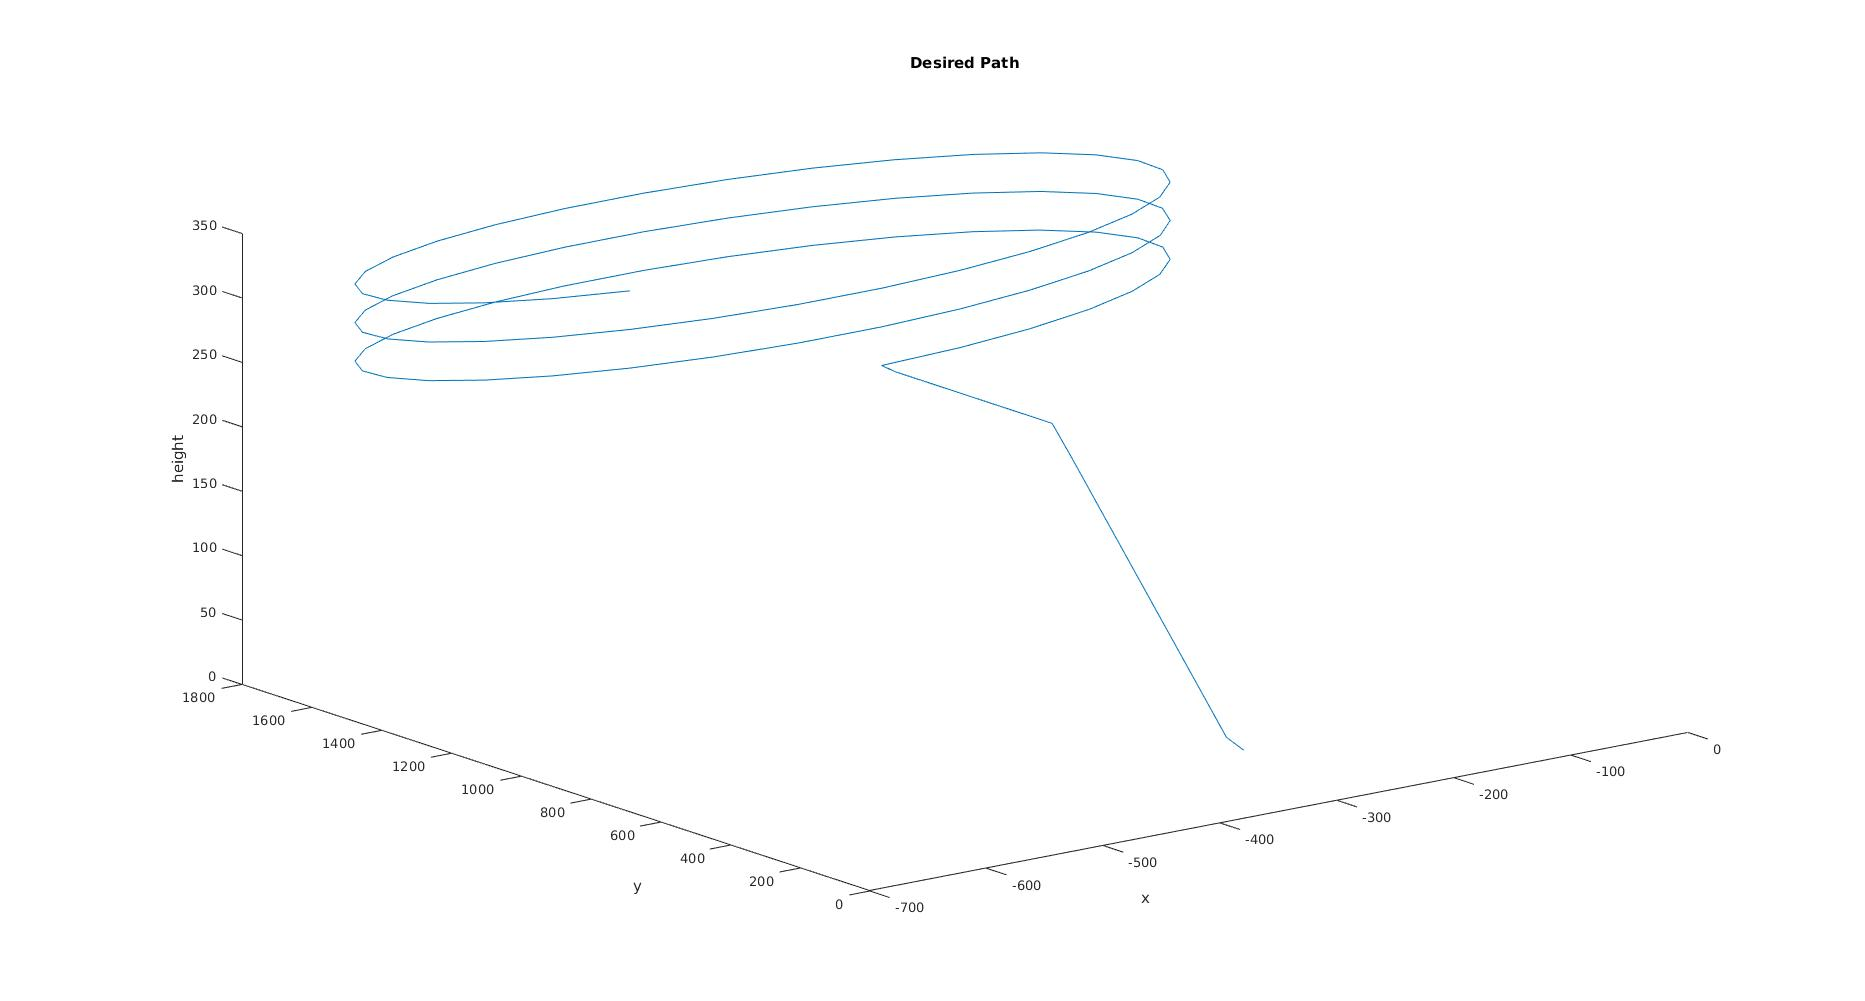
\includegraphics[width=16cm]{pictures/Results/Circle-desired.jpg}
  	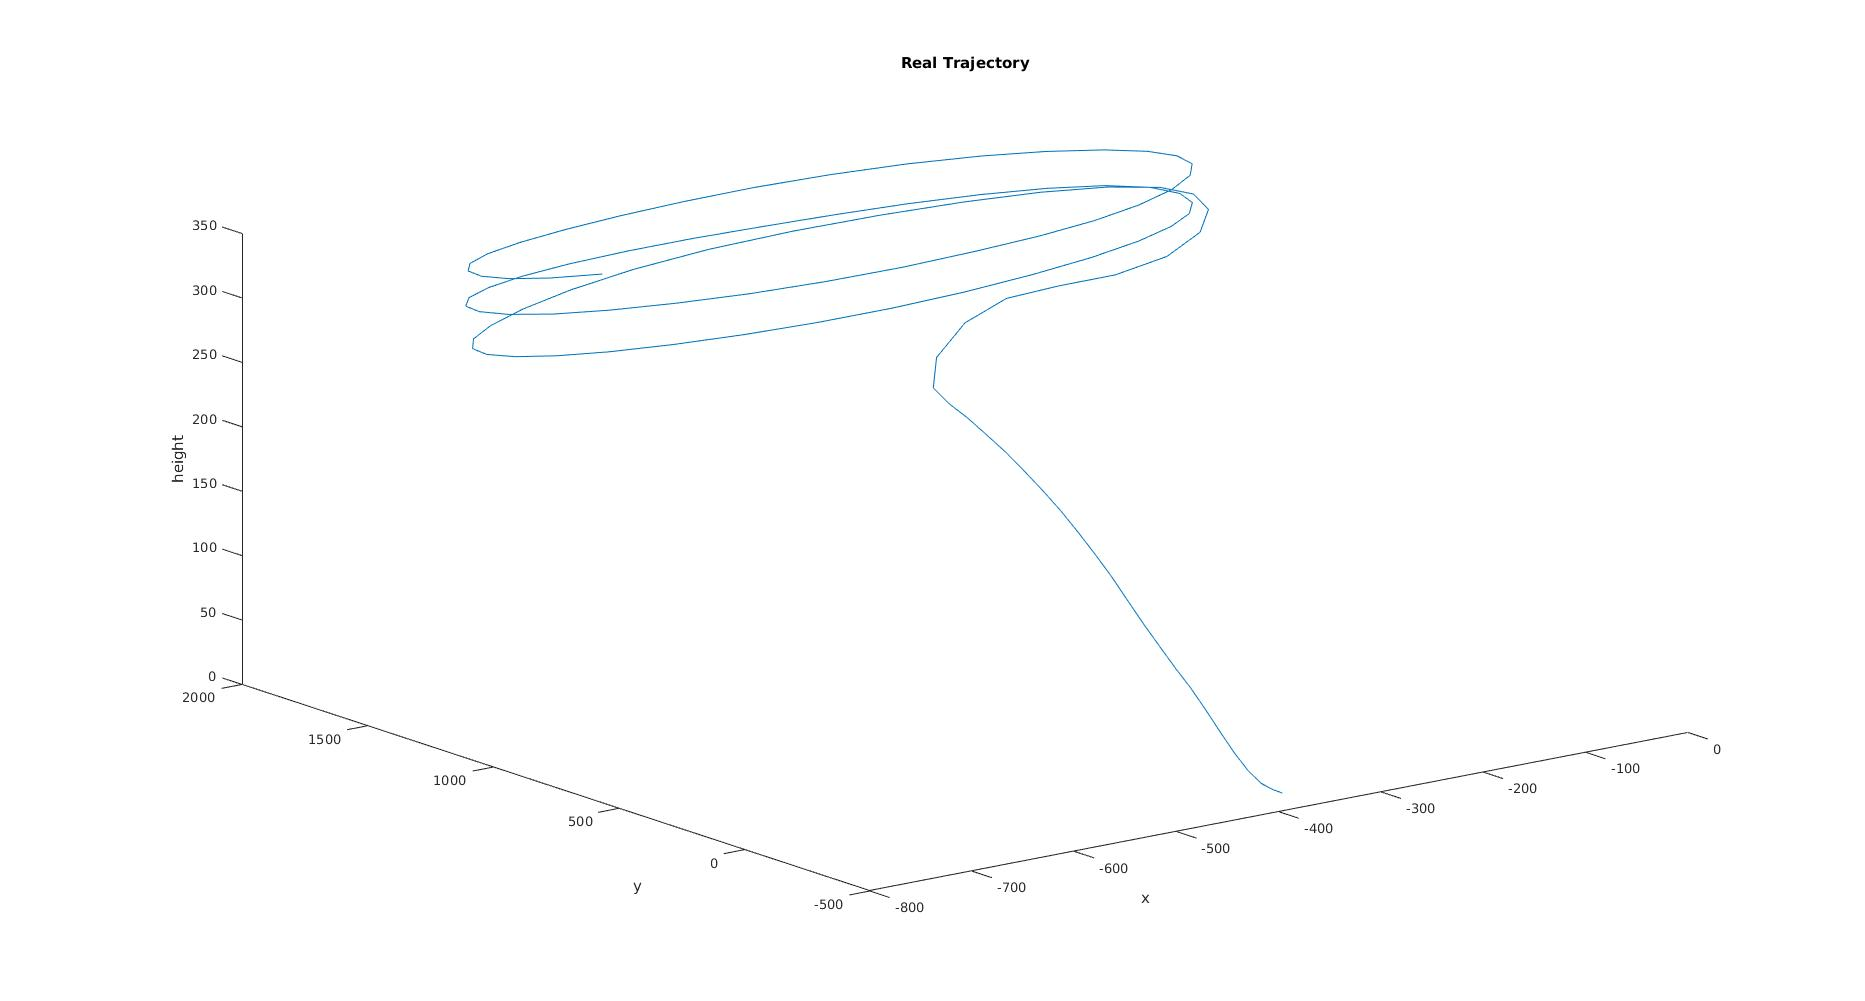
\includegraphics[width=16cm]{pictures/Results/Circle-real.jpg}
  \caption{Comparison of desired and real trajectories of circle flights.}
  \label{fig_circle}
\end{figure}

\begin{figure}[!h]
  \centering
  	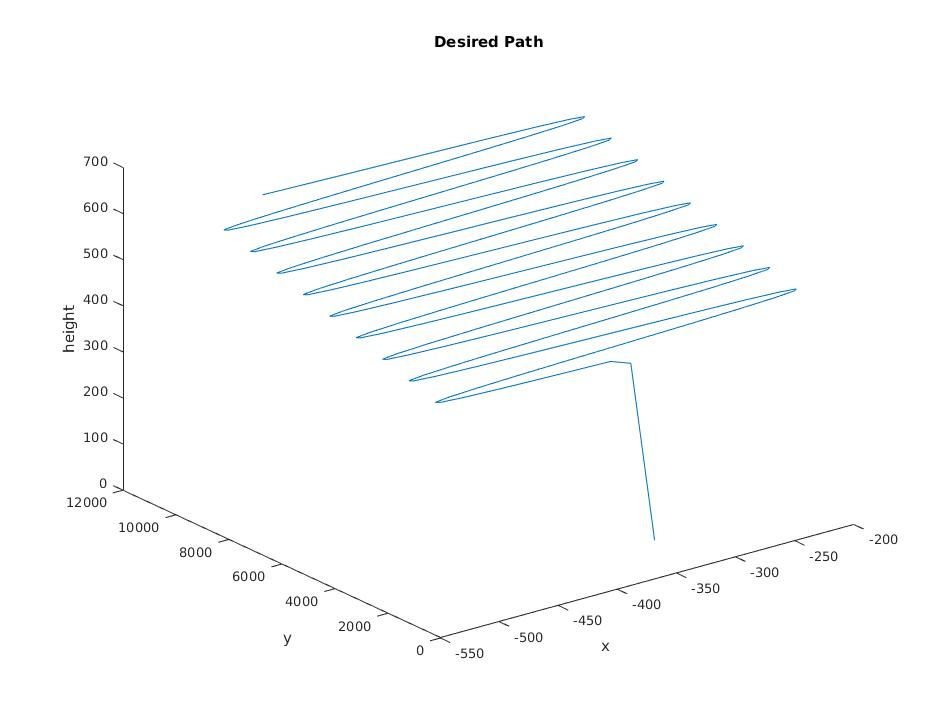
\includegraphics[width=13cm]{pictures/Results/snake-desired.jpg}
  	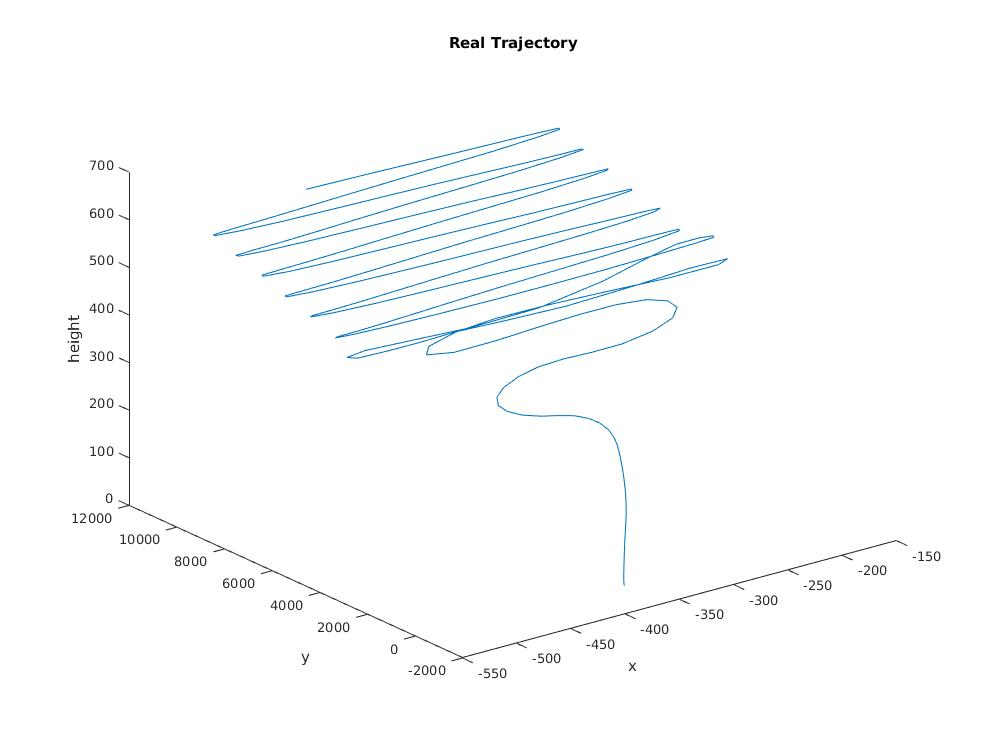
\includegraphics[width=13cm]{pictures/Results/snake-real.jpg}
  \caption{Comparison of desired and real trajectories of snake flights.}
  \label{fig_snake}
\end{figure}			

\begin{figure}[!h]
  \centering
  	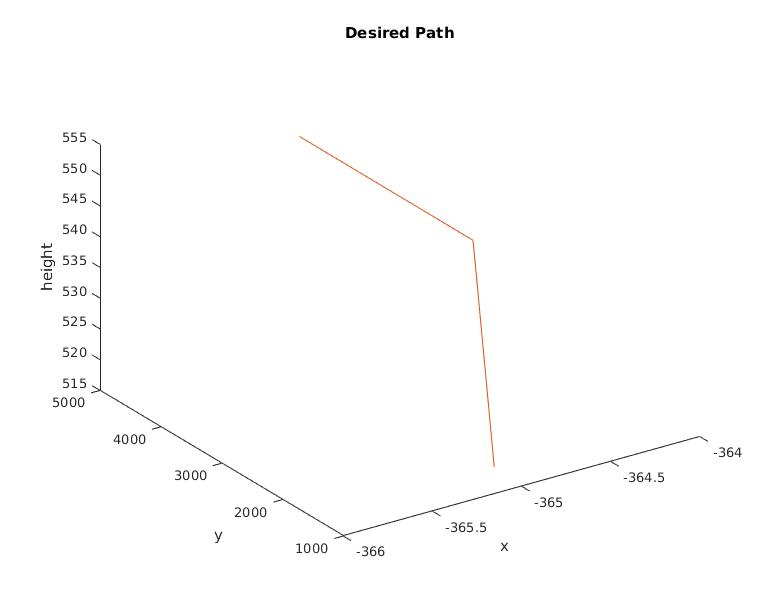
\includegraphics[width=13cm]{pictures/Results/roll-desired.jpg}
  	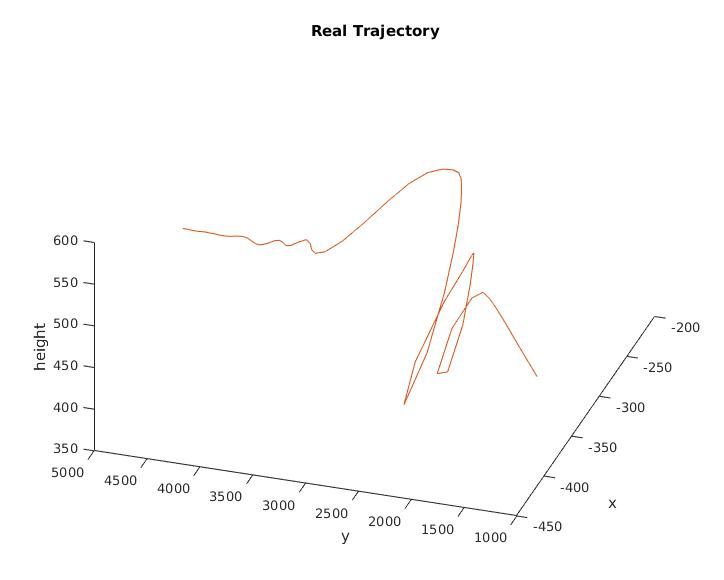
\includegraphics[width=13cm]{pictures/Results/roll-real.jpg}
  \caption{Comparison of desired and real trajectories of rolling flights.}
  \label{fig_roll}
\end{figure}		


\FloatBarrier

% Textende
%----------------------------------------------------------------
%----------------------------------------------------------------
% Anhang

\newpage

\begin{appendix}
%\renewcommand{\refname}{A}
\section{Appendix}

\bigskip



% Literatur
% ===========================================
\subsection{References}

\begin{flushleft}
\renewcommand{\refname}{}
\singlespacing
%\bibliography{references}
{\def\section*#1{}\bibliography{references}}
\end{flushleft}

%\newpage


\bigskip

\subsection{Notation}

\begin{tabbing}
	 \hspace{2cm} \= \hspace{2cm} \= \hspace{3cm} \kill
	\> $t_k$ \> Point in time (time-discrete)\\	
	\> $\Delta T$ \> Time period of one time step of the system\\
	\> $\phi_{ref}$ \> Angle of reference vector for aileron control, forces the roll-angle\\
	\> $\vec{P}_{des}^i$ \> Desired position of the aircraft (inertial frame)\\
	\> $\vec{P}_{is}^i$ \> Actual position of the aircraft (inertial frame)\\
	\> $\vec{L}_{is}^i$ \> Difference between desired and actual position (inertial frame)\\
	\> $\vec{a}_{CMD}^v$ \> Desired Acceleration of the aircraft (vehicle frame)\\
	\> $\vec{g}^{v,b}$ \> Acceleration by gravity (vehicle,body frame)\\
	\> $\vec{A}_{CMD}^{v,b}$ \> Desired Acceleration with gravity considered (vehicle,body frame)\\
	\> $L_{des}$ \> Look-ahead distance \\
	\> $L_{is,Path}$ \> Distance concerning the desired path, the aircraft lags behind \\
	\> $\Delta L$ \> Desired distance the aircraft needs to catch up \\
	\> $e_{Throttle}$ \> Input error for the throttle controller \\
	\> $(\phi,\theta,\psi)$ \> Euler angles of the aircraft \\
	\> $\vec{V}^v$ \> Velocity vector of the aircraft (vehicle frame)\\	
	
\end{tabbing}


\end{appendix}

\end{document}


% -------------------Bausteine--------------------------------------
	
%\begin{figure}[!b]
%  \begin{center}
%    \includegraphics[width=16cm]{../Machine-Epsilon-different-divisors.eps}
%  \end{center}
%  \caption{\small Figure caption. To get a figure to span two
%      columns, use the environment figure* rather than figure.}
%  \label{fig-label}
%\end{figure}


%\begin{enumerate}[{(\arabic{enumi})}]
%
%	\item
%			
%\end{enumerate}

%\begin{pspicture}[xAxisLabel=Auslastung,yAxisLabel=Herst.-Kosten](-0.5,0)(0.5,6.5)
%\begin{psgraph}[arrows=->,Dx=1,Dy=2](0,0)(-0.1,-0.1)(1.2,1.2){5cm}{4cm}
%	\psplot[plotpoints=200,linecolor=red]{0.075}{1}{0.2 0.1 x add div}
%\end{psgraph}
%\end{pspicture}

%\begin{figure}[ph]
%	\centering
%	\caption{Function with three different solvers for task~2.}
%	\lstinputlisting{../Solver.m}
%	\label{Code-Solver}
%\end{figure}

	
%\section{Literature}
%
%\renewcommand{\refname}{}
%
%\begin{flushleft}
%
%\singlespacing
%\bibliography{references}
%
%\end{flushleft}

%\begin{figure}[ph]
%	\centering
%	\subfloat[Forward Euler]{
%		\includegraphics[width=7.5cm]{../02-FE.eps}
%	}
%	\hfill
%	\subfloat[Symplectic Euler]{
%		\includegraphics[width=7.5cm]{../02-SE.eps}
%	}
%	\\
%	\centering
%	\subfloat[Stormer-Verlet]{
%		\includegraphics[width=7.5cm]{../02-SV.eps}
%	}
%	\hfill
%	\subfloat[Monat November]{
%		\includegraphics[width=7.5cm]{../02-err.eps}
%	}
%	\hfill
%	\caption{Solutions of the computed methods in task~2.}
%	\label{02}
%\end{figure}

%\renewcommand{\arraystretch}{1.4}
%\begin{table}[ht]
%\caption{Simulierte Szenarien.}
%\centering
%\begin{tabular}{R{5cm}|cc}
%\toprule 
%\textbf{Größe} & \textbf{Formelzeichen} & \textbf{Einheit} \\
%\midrule
%\textbf{Strahlungsfluss} & $\Phi_e$ & $\SI{}{\watt}$ \\
%\textbf{Bestrahlungsstärke} & $E_e = \frac{\mathrm d \Phi_e}{\mathrm d A}$ & $\SI{}{\watt \per \square \meter}$ \\
%\textbf{Lichtstrom} & $\Phi$ & $\SI{}{\lumen}$ \\
%\textbf{Beleuchtungsstärke} & $L = \frac{\mathrm d \Phi}{\mathrm d A}$ & $\SI{}{\lux} = \SI{}{\lumen \per \square \meter}$ \\
%\textbf{Lichtausbeute} & $K = \frac{\Phi}{P}$ & $\SI{}{\lumen \per \watt}$ \\
%\bottomrule 
%\end{tabular}
%\label{tab:groessen-einheiten}
%\end{table}
%\renewcommand{\arraystretch}{1.0}
